\documentclass[tikz,border=10pt]{standalone}
\usepackage{helvet}
\renewcommand{\familydefault}{\sfdefault}
\usepackage{tikz}
\usepackage{amsmath}
\usetikzlibrary{arrows.meta, positioning, calc, shapes.geometric, decorations.pathreplacing, shadows}

\definecolor{emeraldpine}{HTML}{1A4D3E}
\definecolor{harvardcrimson}{HTML}{A51C30}
\definecolor{ethdarkblue}{HTML}{1F407A}
\definecolor{ethpetrol}{HTML}{007A87}
\definecolor{ethbronze}{HTML}{B87333}
\definecolor{ethpurple}{HTML}{5B4B8A}
\definecolor{ink}{HTML}{1A202C}
\definecolor{softink}{HTML}{4A5568}
\definecolor{paleink}{HTML}{A0AEC0}
\definecolor{cardbg}{HTML}{F8FAFC}
\definecolor{shadecolor}{HTML}{F4F6F9}

\begin{document}
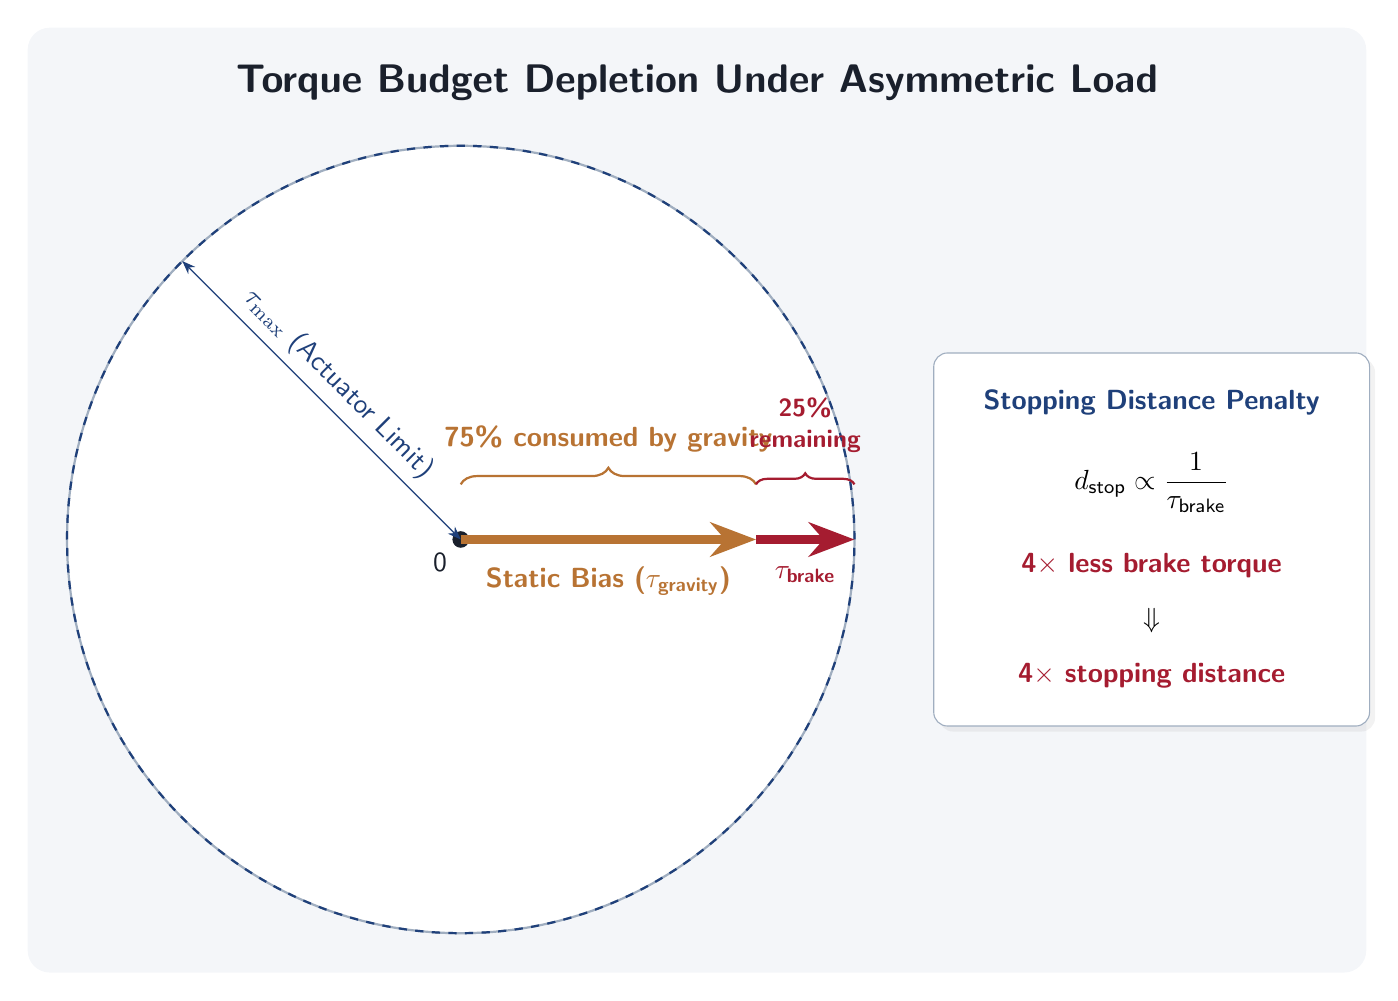
\begin{tikzpicture}[>=Stealth, font=\sffamily]
    % Dimensions
    \def\R{5}
    \def\bias{3.75} % 75% of 5
    
    % Background box
    \fill[shadecolor, rounded corners=8pt] (-5.5, -5.5) rectangle (11.5, 6.5);
    
    % Torque Boundary
    \draw[thick, paleink, fill=white] (0,0) circle (\R);
    \draw[thick, ethdarkblue, dashed] (0,0) circle (\R);
    
    % Center origin
    \fill[ink] (0,0) circle (3pt) node[below left=2pt] {0};
    
    % Radius Label
    \draw[<->, ethdarkblue, thin] (0,0) -- ({-\R*cos(45)}, {\R*sin(45)}) node[midway, sloped, above] {$\tau_{\max}$ (Actuator Limit)};
    
    % Vectors
    \draw[->, line width=3pt, ethbronze] (0,0) -- (\bias, 0) node[midway, below=5pt, font=\bfseries] {Static Bias ($\tau_{\text{gravity}}$)};
    \draw[->, line width=3pt, harvardcrimson] (\bias,0) -- (\R, 0) node[midway, below=5pt, font=\bfseries] {$\tau_{\text{brake}}$};
    
    % Braces
    \draw[decorate, decoration={brace, amplitude=6pt}, thick, ethbronze] 
        (0, 0.7) -- (\bias, 0.7) node[midway, above=8pt, font=\bfseries] {75\% consumed by gravity};
    
    \draw[decorate, decoration={brace, amplitude=4pt}, thick, harvardcrimson] 
        (\bias, 0.7) -- (\R, 0.7) node[midway, above=8pt, font=\small\bfseries, align=center] {25\% \\ remaining};
        
    % Right panel
    \node[anchor=west, fill=white, draw=paleink, rounded corners=5pt, inner sep=12pt, drop shadow={opacity=0.1, shadow xshift=2pt, shadow yshift=-2pt}] at (6.0, 0) {
        \begin{tabular}{c}
            \textbf{\textcolor{ethdarkblue}{Stopping Distance Penalty}} \\[12pt]
            $d_{\text{stop}} \propto \dfrac{1}{\tau_{\text{brake}}}$ \\[18pt]
            \textcolor{harvardcrimson}{\textbf{4$\times$ less brake torque}} \\[8pt]
            $\Downarrow$ \\[8pt]
            \textcolor{harvardcrimson}{\textbf{4$\times$ stopping distance}}
        \end{tabular}
    };
    
    % Title
    \node[font=\Large\bfseries, ink] at (3.0, \R + 0.8) {Torque Budget Depletion Under Asymmetric Load};

\end{tikzpicture}
\end{document}
